%%%%%%%%%%%%%%%%%%%%%%%%%%%%%%%%%%%%%%%%%%%%%%%%%%%%%%%%%%%%%%%%%%%%
%% I, the copyright holder of this work, release this work into the
%% public domain. This applies worldwide. In some countries this may
%% not be legally possible; if so: I grant anyone the right to use
%% this work for any purpose, without any conditions, unless such
%% conditions are required by law.
%%%%%%%%%%%%%%%%%%%%%%%%%%%%%%%%%%%%%%%%%%%%%%%%%%%%%%%%%%%%%%%%%%%%

% This theme was based on fibeamer theme 
% If you found any bugs please contact @karlosos
% This repository is hosted on github https://github.com/karlosos/zut-fibeamer/

\documentclass{beamer}
\usetheme[faculty=wi]{fibeamer}
\usepackage[utf8]{inputenc}
\usepackage[
  main=polish,
  polish
]{babel}

\title{Aula 5  - Datas}
\subtitle{Tópicos especiais em Sistemas}
\author{Prof. Juliana Costa Silva - juliana.silva@up.edu.br}

\usepackage{ragged2e}  % `\justifying` text
\usepackage{booktabs}  % Tables
\usepackage{tabularx}
\usepackage{tikz}      % Diagrams
\usetikzlibrary{calc, shapes, backgrounds}
\usepackage{amsmath, amssymb}
\usepackage{url}       % `\url`s
\usepackage{listings}  % Code listings
\frenchspacing
\begin{document}

%------------------------------------------------------------------------
  \frame[c]{\maketitle}
      \begin{frame}<beamer>
      \frametitle{O que veremos hoje}
      \tableofcontents
    \end{frame}
%------------------------------------------------------------------------
    \section{Revendo...}
    \begin{frame}{Revendo...}{O que já aprendemos?}
      
      \begin{itemize}
            \item Criamos um projeto node;
            \item organizamos os arquivos de configuração na pasta config;
            \item Organizamos os controladores na pasta controllers;
            \item Configuramos ações de GET e POST para a rota \alert{movimento}.
            \item Enviamos dados em formato JSON
             \item Persistência de dados
       \end{itemize}
     \end{frame}
     %------------------------------------------------------------------------
\begin{frame}[label=proof]{O projeto da disciplina}
	\begin{itemize}
	\item Faremos um sistema de controle financeiro pessoal;
	\item Este sistema deve ter:
	\begin{itemize}
	\item Registro de gastos;
	\item Login de usuários;
	\item Registro de renda (salários - comissões - negócios);
	\item Registro de cartões de créditos;
	\item Registro de contas bancárias;
	\end{itemize}
	\end{itemize}
    \end{frame}
%------------------------------------------------------------------------
    \begin{frame}[label=lists]{Trabalhando com datas}
      \begin{columns}[onlytextwidth]
        \column{.5\textwidth}
          \begin{itemize}
            \item Vamos acrescentar a data de registro do movimento no sistema;
            \item Também vamos acrescentar a data em que o usuário declara o movimento;
            \item Ou seja, dataCriacao é registrada automaticamente pela aplicação, já data é informada pelo usuário;
          \end{itemize}
        \column{.5\textwidth}
            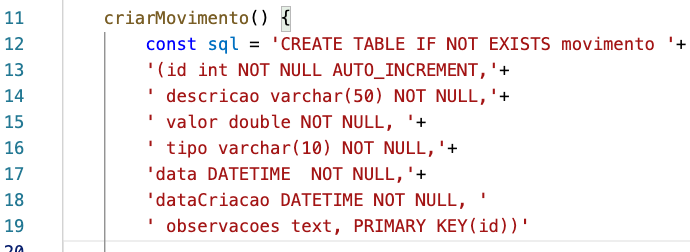
\includegraphics[width=60mm]{resources/aula9_2.png}\\
            \tiny{Novo script de criação de tabela}
      \end{columns}
    \end{frame}

%------------------------------------------------------------------------
\section{Conversão}
    \begin{frame}[label=lists]{Recebendo datas}
    \begin{exampleblock}{formatos de datas}
        	\begin{itemize}
	\item Ao digitaros datas (no Brasil) utilizamos o formato DD-MM-AAAA
	\item Porém no banco de dados as datas são registradas num padrão diferente;
	\item Vamos instalar bibliotecas para tratamento de datas; \textbf{conncetion.js}.
        	\end{itemize}
      \end{exampleblock}
    \end{frame}
%------------------------------------------------------------------------
    \begin{frame}[label=lists]{Instalação moment}

% \begin{columns}[onlytextwidth]
%        \column{.5\textwidth}
         Para realizar a instalação da biblioteca moment use o comando \alert{npm install moment}
         \begin{itemize}
         \item No arquivo \textbf{models/movimento.js};
         \item Adicionaremos a data ao objeto movimento
         \end{itemize}
%        \column{.5\textwidth}
	            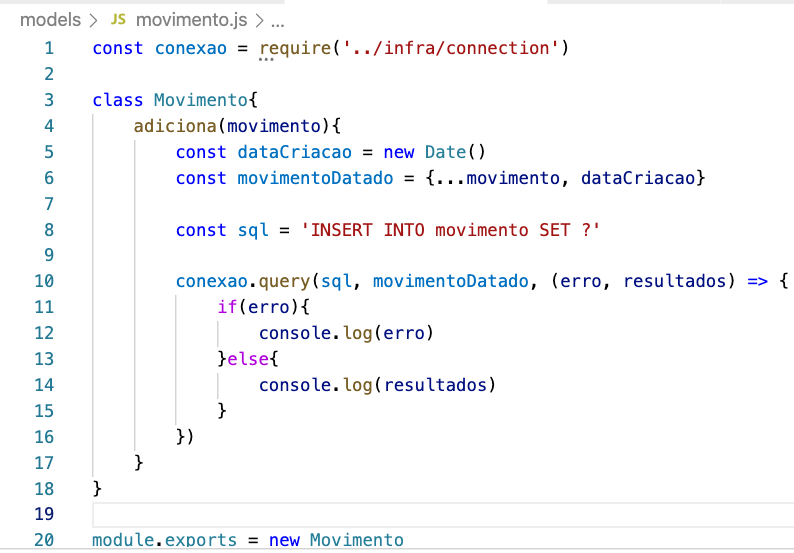
\includegraphics[width=80mm]{resources/aula9_1.png}\\
            \tiny{\textbf{Fonte:} O autor}
%      \end{columns}
    \end{frame}

%------------------------------------------------------------------------
    \begin{frame}[label=lists]{Adicionando datas}
      \begin{columns}[onlytextwidth]
        \column{.5\textwidth}
          \begin{itemize}
            \item Criamos uma constante dataCriacao que recebe a data e hora do sistema ao ser instanciada;
            \item O objeto movimentoDatado é um array que incorpora todo o objeto movimento + data;
            \item O valor do campo data será recebido pelo JSON;
          \end{itemize}
        \column{.5\textwidth}
            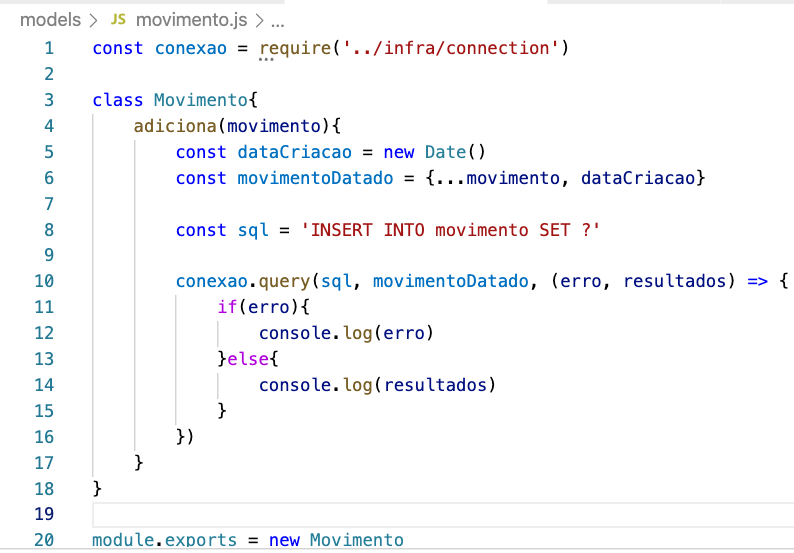
\includegraphics[width=60mm]{resources/aula9_1.png}\\
            \tiny{Novo script da classe Movimento}
      \end{columns}
    \end{frame}
%------------------------------------------------------------------------
% \subsection{Referências}
%    \begin{frame}{Referências}%[allowframebreaks]
%\frametitle{Referências}
%\small
%\begin{center}
%\tiny
%\bibliographystyle{apalike}
%\bibliography{./ref_aula}
%\end{center}
%\end{frame}
  
\end{document}
